\documentclass[10pt,a4paper]{article}
\usepackage[utf8]{inputenc}
\usepackage{amsmath}
\usepackage{gensymb}
\usepackage{amsfonts}
\usepackage{siunitx}
\usepackage[european]{circuitikz}
\usepackage{geometry}
\newgeometry{tmargin=2cm, bmargin=2cm, lmargin=2cm, rmargin=2cm}
\usepackage{amssymb}
\usepackage{multirow}
\usepackage{polski}
\usepackage{graphicx}
\author{\textbf{T. Fąs}}
\title{\textbf{BADANIE WIDMA LINIOWEGO}}
\begin{document}
\maketitle

\begin{center}
\textbf{\subsection*{STRESZCZENIE}}
\end{center}
W doświadczeniu wyznaczono zależność współczynników załamania światła od długości fali dla w uproszczonym modelu Sellmeiera postaci $n^2-1=B\lambda^2/(\lambda^2-C)$. Otrzymano wartości: $B=1,7447\pm0,0011$ 1/nm$^2$, $C=20091\pm141$ nm$^2$.


\begin{center}
\textbf{\subsection*{WSTĘP}}
\end{center}

\begin{figure}[h!]
\centering
\begin{minipage}{0.5\textwidth}
  \centering
  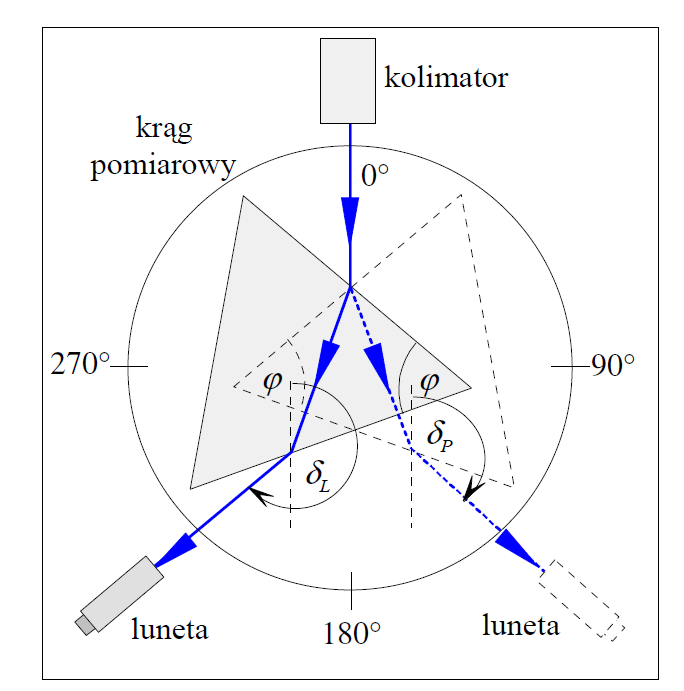
\includegraphics[width=6cm, height=5cm ]{rap13ukl1} 
\caption{Wyznaczanie kąta najmniejszego odbicia.}
\end{minipage}%
\begin{minipage}{0.5\textwidth}
  \centering
  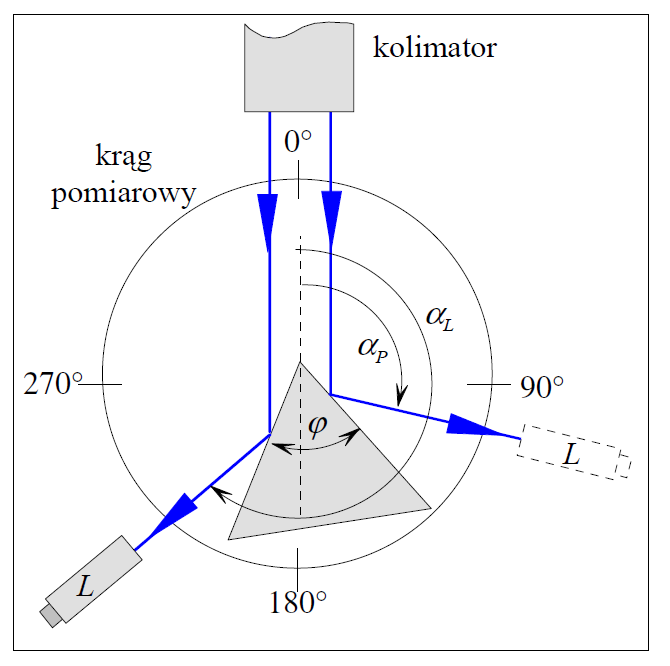
\includegraphics[width=6cm, height=5cm ]{rap13ukl2} 
\caption{Wyznaczanie kąta łamiącego.}
\end{minipage}
\end{figure}


Jeżeli promień pada na pryzmat tak, jak na Rysunku 1, to współczynnik załamania $n$ można wyznaczyć, korzystając z prawa Snella. Jeżeli znamy kąt najmniejszego odbicia $\delta$ oraz kąt łamiący pryzmatu $\varphi$, to $n$ wyrażone jest wzorem:
\begin{equation}
n=\dfrac{\sin\left(\dfrac{1}{2}\left(\delta+\varphi\right)\right)}{\sin\left(\dfrac{1}{2}\varphi\right)},
\end{equation}
przy czym zachodzi równość:
\begin{equation}
\delta=\dfrac{1}{2}\left(\delta_{l}-\delta_{p}\right).
\end{equation}
Z kolei z Rysunku 2 wynika, iż kąt łamiący pryzmatu można wyznaczyć ze związku 
\begin{equation}
\varphi=\dfrac{1}{2}\left(\alpha_{l}-\alpha_{p}\right).
\end{equation}

 Jeżeli znane są rożne wartości współczynników $n$ dla rożnych długości fali $\lambda$, to można do tych danych dopasować zależność:
\begin{equation}
n=A_{0}+\dfrac{A_{1}}{\lambda^2},
\end{equation}
lub
\begin{equation}
n^2-1=\dfrac{B\lambda^2}{\lambda^2-C},
\end{equation}
przy czym $A$, $B$, $C$ to współczynniki dopasowania.

Znając współczynniki dopasowania, można odwrócić powyższe zależności, by na podstawie kąta najmniejszego odbicia móc określić długość fali światła. To właśnie wyznaczenie zależności długości fali od kąta odbicia było celem tego doświadczenia.
 
\begin{center}
\textbf{\subsection*{UKŁAD DOŚWIADCZALNY}}
\end{center}

Do pomiarów kątów skorzystano z goniometru, a źródłem światła była lampa wodorowa, helowa i neonowa. Goniometr wraz ze szklanym pryzmatem był w trakcie pomiarów ustawiany zgodnie z Rysunkiem 1 i Rysunkiem 2. W trakcie szukania kąta najmniejszego odbicia pryzmat był obracany tak, jak wskazuje na to Rysunek 2, przy czym sam kąt rozpoznawano po tym, że w trakcie obrotu dochodziło w pewnym momencie do cofania się obrazy widma. 

\begin{center}
\textbf{\subsection*{WYNIKI POMIARÓW}}
\end{center}
Zmierzono: $\alpha_{p}=125^{\circ}11'$, $\alpha_{l}=214^{\circ}28'$. Tabela 1 przedstawia pomiary kątów $\delta_{l}$ i $\delta_{p}$ wraz z powiązanymi z nimi długościami fali. Cztery pierwsze długości fali to widmo helu, a trzy kolejne to widmo wodoru.

\begin{table}[h!]
\centering
\caption{Kąty załamania.}
\begin{tabular}{|c|c|c|c|c|c|c|c|}
\hline
Długość fali $\lambda$ [nm] & 667,8          & 587,5          & 504,7          & 447,1          & 656,3          & 486,1           & 434,0          \\ \hline
Kąt $\delta_{p}$            & 145$^\circ$18' & 144$^\circ$53' & 144$^\circ$09' & 143$^\circ$24' & 145$^\circ$13' & 143$^\circ$59'  & 143$^\circ$10' \\ \hline
Kąt $\delta_{l}$            & 214$^\circ$16' & 215$^\circ$10' & 215$^\circ$53' & 216$^\circ$37' & 214$^\circ$48' & 216$^\circ$ 05' & 216$^\circ$53' \\ \hline
\end{tabular}
\end{table}

Oprócz tego dokonano pomiarów kąta załamania $\delta$ przy stałej pozycji pryzmatu. Pozwala to na bezpośrednie wyznaczenie zależności kąta od długości fali. Wyniki tych pomiarów przedstawione są w Tabeli 2.


\begin{table}[h!]
\centering
\caption{Kąty załamania: stała pozycja pryzmatu.}
\begin{tabular}{|c|c|c|c|c|c|c|c|}
\hline
Długość fali $\lambda$ [nm] & 667,8          & 587,5          & 504,7          & 447,1          & 656,3          & 486,1          & 434,0          \\ \hline
Kąt $\delta$                & 141$^\circ$17' & 140$^\circ$54' & 140$^\circ$15' & 139$^\circ$35' & 141$^\circ$13' & 140$^\circ$05' & 139$^\circ$23' \\ \hline
\end{tabular}
\end{table}

Dokonano też pomiarów widma neonu. Zdecydowano się na wybór wyraźnie widocznej linii światła żółtego, któremu odpowiadają kąty: przy pierwszym pomiarze $\delta_{p}=145^\circ9'$, $\delta_{l}=215^\circ53'$; przy pomiarze ze stałą pozycją pryzmatu: $\delta=140^\circ51'$. Kąty te odpowiadają długości fali 588,2 nm.

Wyniki pomiarów dla krawędzi światła białego wyglądają następująco: dla światła czerwonego  $\delta_{p}=145^\circ20'$, $\delta_{l}=214^\circ38'$, $\delta=141^\circ19'$; dla fioletu: $\delta_{p}=142^\circ38'$, $\delta_{l}=217^\circ39'$, $\delta=138^\circ59'$.

\begin{center}
\textbf{\subsection*{ANALIZA DANYCH}}
\end{center}
Niepewność pomiarów wszystkich kątów oszacowano na $\Delta=1'$, ponieważ widoczne linie były na tyle cienkie, że uchwycenie momentu cofania się obrazu, jak i precyzyjne wyznaczenie pozycji linii nie stanowiło większego problemu.

Aby przenieść te niepewności na niepewności kąta łamiącego i kąta najmniejszego odchylenia, skorzystano z metody propagacji małych błędów. Ogólny wzór przenoszenia niepewności w tej metodzie jest następujący:

 \begin{equation}
 u_{f}^2=\sum_{i=1}^n \left( \dfrac{\partial f}{\partial x_{i}}u_{i}\right)^2+\sum_{i=1, i\neq j}^n \left( \dfrac{\partial f}{\partial x_{i}}\dfrac{\partial f}{\partial x_{j}}c_{ij}\right),
 \end{equation}
 gdzie wielkość $f$ zależy od wielkości $x_{i}$ o niepewnościach $u_{i}$ i o ocenach kowariancji $c_{ij}$ \cite{tay1}. W przypadku mierzonych kątów, kowariancja między nimi wynosi 0.

Stosując dane z Tabeli 1 oraz Równanie (6) wyznaczono kąt łamiący pryzmatu $\varphi=(44,642\pm0,012)^\circ$ oraz współczynniki załamania $n$ wraz z ich niepewnościami $u_{n}$. Wyniki umieszczono w Tabeli 3.

\begin{table}[h!]
\centering
\caption{Współczynniki załamania i ich niepewności.}
\begin{tabular}{|c|c|c|c|c|c|c|c|}
\hline
Długość fali $\lambda$ [nm] & 667,8 & 587,5 & 504,7 & 447,1 & 656,3 & 486,1 & 434,0 \\ \hline
Współczynnik $n$            & 1,681 & 1,689 & 1,701 & 1,714 & 1,682 & 1,705 & 1,719 \\ \hline
Niepewność $u_{n}$          & 0,029 & 0,030 & 0,030 & 0,030 & 0,029 & 0,030 & 0,030 \\ \hline
\end{tabular}
\end{table}


W następnym kroku, korzystając z programu \textit{gnuplot} wykonano dopasowanie danych z Tabeli 3 zgodnie z Równaniem (4) oraz Równaniem (5) Krzywe najlepszego dopasowania są przedstawione na Rysunku 3 i Rysunku 4, a parametry dopasowania wraz z ich niepewnościami $u_{i}$ przedstawione są w Tabeli 4.


\begin{figure}[h!]
\centering
\begin{minipage}{0.5\textwidth}
  \centering
  \includegraphics[width=8cm, height=5cm ]{rap15rys1} 
\caption{Dopasowanie danych: model Cauchy.}
\end{minipage}%
\begin{minipage}{0.5\textwidth}
  \centering
  \includegraphics[width=8cm, height=5cm ]{rap15rys2} 
\caption{Dopasowanie danych: model Sellmeiera.}
\end{minipage}
\end{figure}

\begin{table}[h!]
\centering
\caption{Parametry dopasowania.}
\begin{tabular}{|c|c|c|c|c|}
\hline
Parametr   & $A_{0}$ & $A_{1}$ [nm$^2$] & $B$ [1/nm$^2$] & $C$ [nm$^2$] \\ \hline
Wartość    & 1,65416 & 12053            & 1,7447         & 20091        \\ \hline
Niepewność & 0,00057 & 148              & 0,0011         & 141          \\ \hline
\end{tabular}
\end{table}

Wartości $\chi^2$ wynoszą 0,0012 oraz 0,00044 kolejno dla modelu Cauchy i Sellmeiera.
Otrzymane wartości $\chi^2$ sugerują, iż zależność wyrażona Równaniem (5), czyli model Sellmeiera, jest lepszym odwzorowaniem faktycznie uzyskiwanych wyników.

Odwrócona zależność Sellmeiera wyraża się wzorem:

\begin{equation}
\lambda=\sqrt{\dfrac{C\left(1-n^2\right)}{B+1-n^2}}
\end{equation}

Korzystając z Równania (7) można wyznaczyć długość fali na podstawie znajomości współczynnika załamania, z kolei niepewność tej wielkości można obliczyć, korzystając z Równania (6) i kładąc ocenę kowariancji między współczynnikami $c_{BC}=-0,949$.

Aby sprawdzić działanie Równania (7) podstawiono wartość współczynnika załamania zmierzonej linii neonu. Dla $n=1,693\pm0,030$ otrzymano $\lambda=558\pm217$ nm. Wartość ta jest zgodna z wartością tablicową, która wynosi $558,2$ nm. Jednak ogromna niepewność, jaka temu towarzyszy nie napawa optymizmem. Największy wkład do niepewności ma człon stojący przy niepewności współczynnika załamania. Przy założeniu, że znamy $n$ dokładnie, otrzymamy niepewność długości fali równą $0,85$ nm.

Postanowiono wypróbować alternatywną metodę wyznaczania długości fali. Na podstawie danych z Tabeli (2) wykonano wykres zależności kąta załamania od długości fali. Do tych punktów dopasowano zależność przybliżoną postaci: $\delta=a\lambda^2+b\lambda+c$. Wykres wraz z krzywą najlepszego dopasowania znajduje się na Rysunku 5, z kolei parametry dopasowania znajdują się w Tabeli 5.

\begin{figure}[h!]
\includegraphics[width=10cm]{rap15rys3} 
\centering
\caption{Zależność kąta od długości fali.}
\end{figure}


\begin{table}[h!]
\centering
\caption{Parametry dopasowania.}
\begin{tabular}{|c|c|c|c|c|}
\hline
Parametr   & $a$ [1/nm$^2$]      & $b$ [1/nm] & $c$    & $\chi^2$              \\ \hline
Wartość    & -40,0$\cdot 10^{-8}$ & 0,000580   & 2,2564 & \multirow{2}{*}{7,42} \\ \cline{1-4}
Niepewność & 3,0$\cdot 10^{-8}$  & 0,000033   & 0,0090 &                       \\ \hline
\end{tabular}
\end{table}

Tak więc wzór na długość fali w tej metodzie jest następujący:
\begin{equation}
\lambda=\dfrac{-b+\sqrt{b^2-4ac+4a\delta}}{2a}
\end{equation}
Niepewności liczone są z Równania (6), przy czym $c_{ab}=-0,999$, $c_{ac}=0,995$, $c_{bc}=-0,999$. Dla neonu linii neonu otrzymano wartość $\lambda=578,8/pm1,8$ nm. Ta wartość, na mocy testu 3$\sigma$, nie jest zgodna z wartością wzorcową 588,2 nm. Tak więc metoda ta nie zwraca oczekiwanych wyników, ale pozwala na zgrubne oszacowanie szukanej długości fali.

Na podstawie Równania (7) oraz Równania (8) oszacowano krańce światła widzialnego. Z Równania (7) otrzymano przedział $(405:687)$ nm, z kolei z Równania (8) otrzymano $(405:514)$ nm, co jak widać, jest wynikiem bezsensownym. Równanie (7) daje bardzo dobre przybliżenie rzeczywistego przedziału, który wynosi w przybliżeniu $(390:700)$ nm \cite{ba}.





\begin{center}
\textbf{\subsection*{DYSKUSJA WYNIKÓW I WNIOSKI}}
\end{center} 
Wartości otrzymywane za pośrednictwem Równania (7) są wynikami bardzo dobrymi. Jednakże niepewności jakie towarzyszą tym wynikom są niepokojąco duże. Jedyny sposób na ich minimalizację, to niezwykle dokładne pomiary współczynnika załamania. Największym rozczarowaniem są wyniki otrzymywane za pomocą Równania (8), które z bliżej nieznanych powodów nie zwraca wartości oczekiwanych. Prawdopodobnie, jak sugerują pomiary kontrolne, przedział światła widzialnego i kwadratowa postać przybliżenia, równanie to jest słuszne tylko w wąskim wycinku spektrum. Niezależnie od przyczyn rozbieżności wyników, Równanie (8) nie  spełnia oczekiwań i nie może być brane pod uwagę jako formuła kalibracyjna.

\begin{center}
\begin{thebibliography}{9}

 
\bibitem{tay1}
 J. R. Taylor,
 \emph{Wstęp do analizy błędu pomiarowego},
 PWN, Warszawa, 1995, s. 175.
 
\bibitem{ba}
 C. Starr, L. Starr, C. A. Evers, 
 \emph{Biology: Concepts and Applications},
 Thomson, Brooks/Cole, 2006 


 \end{thebibliography}

\end{center}


\end{document}